%%%
%
% $Autor: Wings $
% $Date: 2024-10-31 11:15:45Z $
% $File: file.tex $
% $Version: 1 $
%
% Project: 
%
%%%


\chapter{Entwicklung der Programmlogik}


\subsection{Identifizieren aller Komponenten und Einflussgrößen }
Am Anfang eines jeden Prjektes ist es maßgeblich für den Projekterfolg, alle Komponenten, Parameter und Funktionen eindeutig zu definieren.  Dementsprechend können grafische Übersichten, welche das System aufschlüsseln sinnvoll sein.  
Besonders Mindmaps eignen sich um kategorisch die Komponenten des Systems aufzuzeigen. 

\begin{center}
	\begin{figure}
		%%hier dei xmind \includegraphics{imagefile}
	\end{figure}
\end{center}

\subsection{Entwicklung der Programmlogik }
Um eine effiziente und vorallem eindeutige Verarbeitung von Signalen und Eingaben zu ermöglichen, erweist es sich als sinnvoll eine grafische Übersicht wie ein Flussdiagramm zu erstellen. Diese Grafik kann zudem bei der Programmierung unterstützen. Im Zuge der Entwicklung und Planung eines Systems bietet ein Flussdiagram somit eine strukturierte Darstellung aller relevanten Abläufe und Entscheidungsprozesse. Durch die visuelle Aufbereitung lassen sich komplexe Zusammenhänge leichter nachvollziehen, wodurch sowohl die Implementierung als auch spätere Anpassungen vereinfacht werden.Zusätzlich können potenzielle Fehlerquellen frühzeitig identifiziert und iterativ durch Verbessern der Logik beseitigt werden. Eindeutig dient dieses Diagramm als Blaupause der Programmstruktur und kann somit bereits früh, benötigte Klassen und Funktionen definieren. 
Ein Grafik (vgl. \ref{pic:FlowChart1})  zur übersichtlichen Dartsellung der Programmlogik wurde dementsprechend angefertigt. 

\begin{center}
	\begin{figure}
		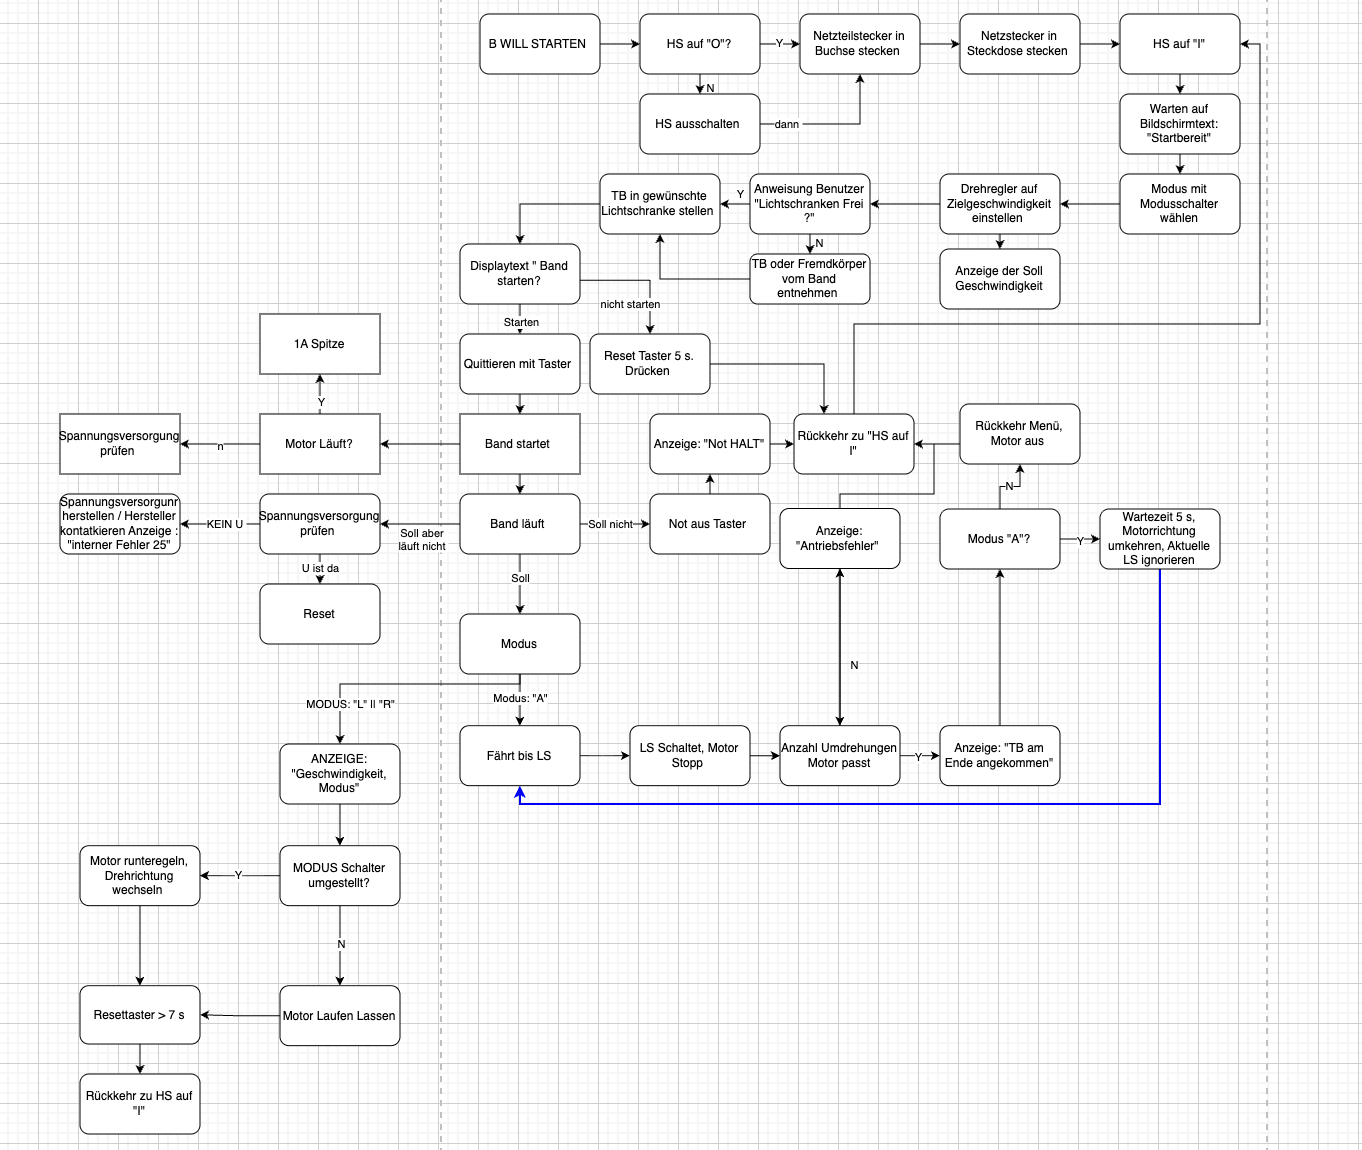
\includegraphics[scale=0.5]{../../Images/Flowchart/FlowChartV1.png}
		\caption{Das Erste Flussdiagramm zur Beschreibung des erzielten Programmablaufes} 
		\label{pic:FlowChart1}
	\end{figure}
\end{center}
Um Fehler zu vermeiden ist es zudem sinnvoll, das System erneut zu entwickeln und grafisch aufzubereiten. Somit wurden die Anforderungen des Systems und seine Komponenten erneut aufgeschlüsselt mithilfe einer MindMap (vgl. \ref{pic:XMind} ) dargestellt.  

\begin{center}
	\begin{figure}
		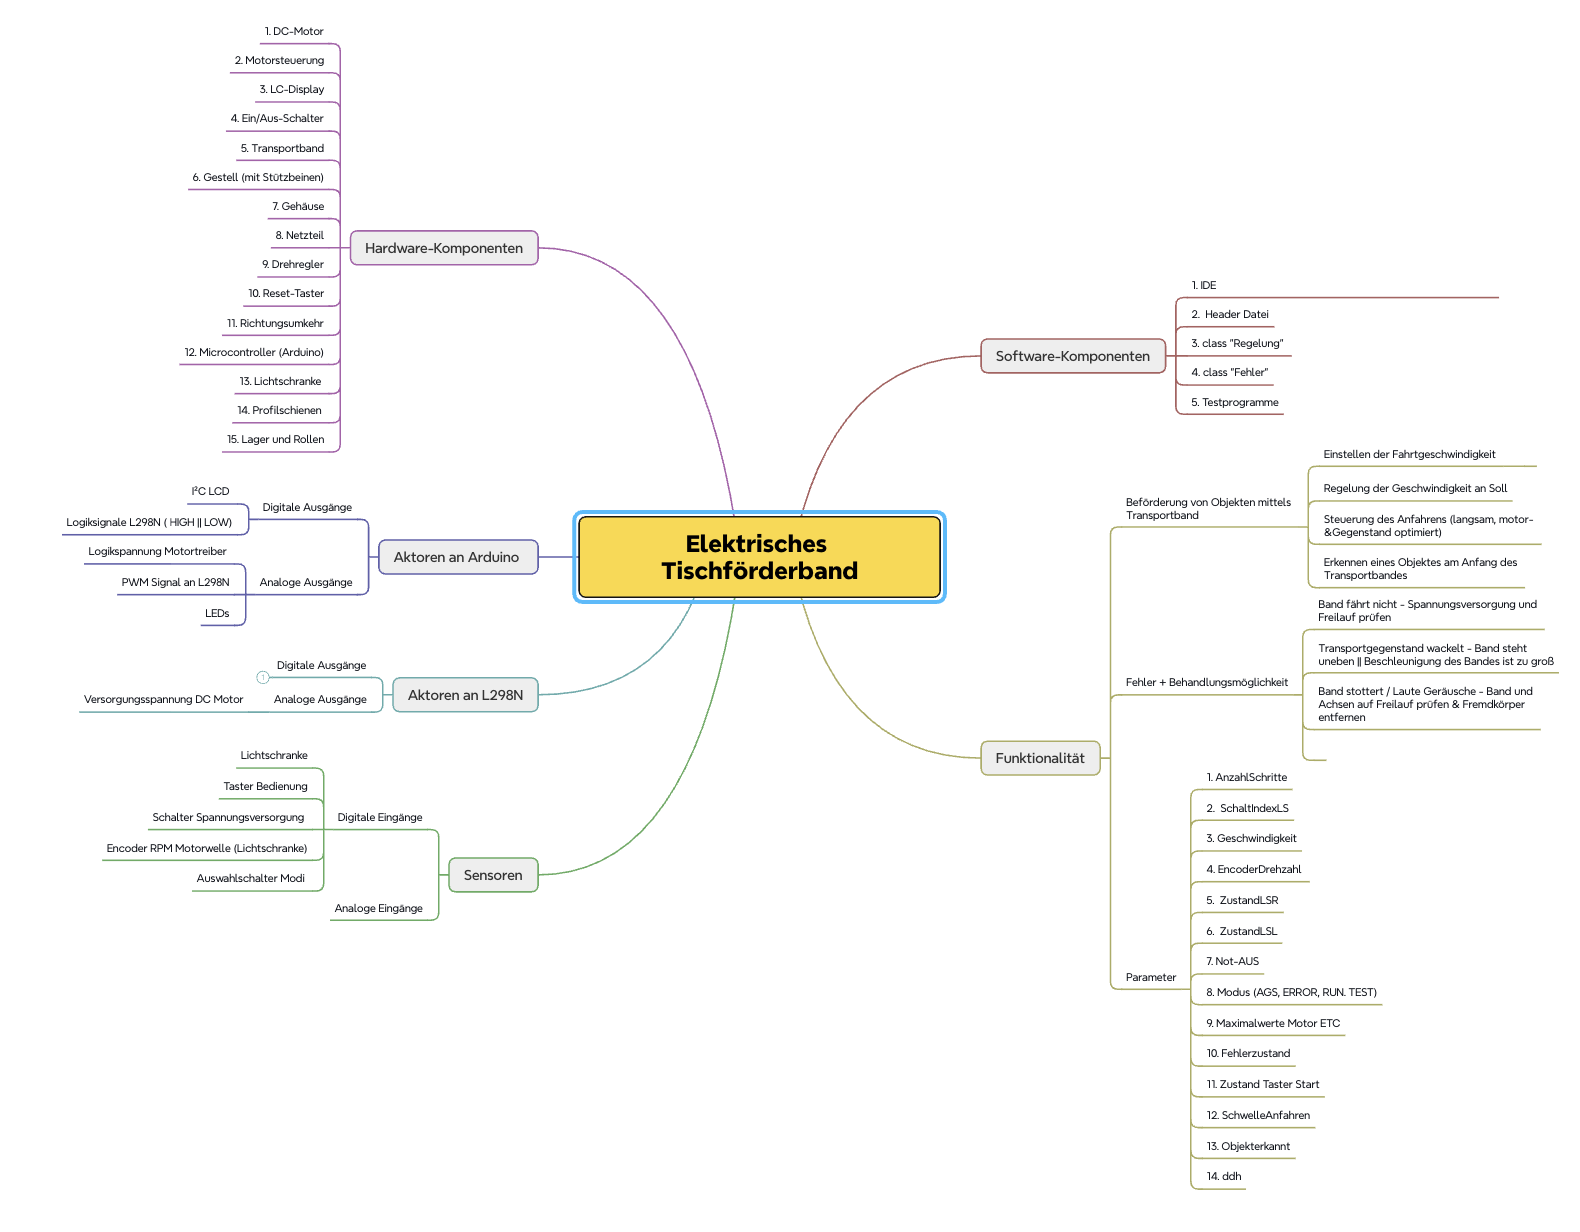
\includegraphics[scale=0.5]{../../Images/Flowchart/Xmind.png}
		\caption{MindMap für alle benötigten Komponenten } 
		\label{pic:XMind}
	\end{figure}
\end{center} 

Aus dieser zweiten Darstellung konnte dann ein neues, überarbeites Flussdiagram erstellt werden. Diese neue Flussdiagramm konnte einige Fehler beseitigen. 
Die verbesserte Version (vgl. \ref{pic:FlowChart2}) des ablauforientierten Flussdiagrammes ist zudem farblich charakterisiert, und zeigt die einzelnen Sequenzen der Bedienung, welcher der Nutzer durchläuft übersichtlich und strukturiert auf. 

\begin{center}
\begin{figure}
	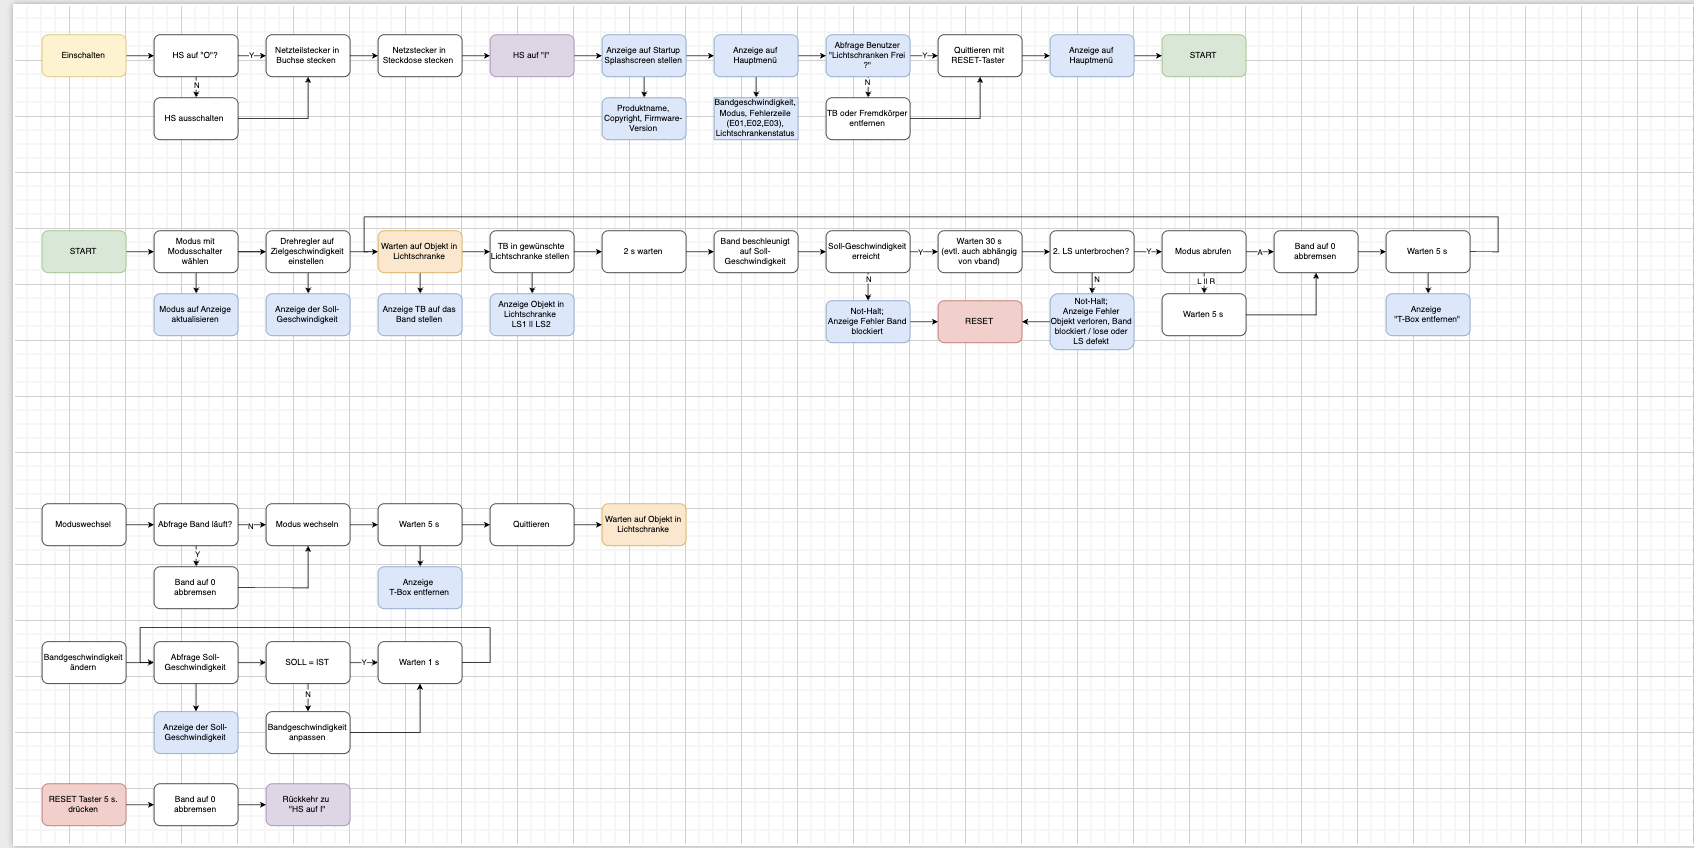
\includegraphics[scale=0.5]{../../Images/Flowchart/Flowchart2.png}
	\caption{Zweite Version des Flussdiagramms, ablauforientiert sowie mit Farblicher Hervorhebung einzelner Seuqenzen } 
	\label{pic:FlowChart2}
\end{figure}
\end{center}   
Für den Aufbau der Ansteureung auf Softwareseite eignet sich eine objektorientierte Programmierung, da diese mit geringem Aufwand angepasst werden kann. Hierfür wurden folgende Klassen definiert :  
\begin{center}
	\begin{enumerate}
		\item \textbf{display.cpp}: Diese Klasse steuert die gesamte Kommunikation zwischen Mikrocontroller und Display. Zudem werden alle Ausgaben des Displays hier konfiguriert und gesteuert. 
		\item \textbf{fehler.cpp}: Diese Klasse ist verantwortlich für das gesamte Fehlermanagement. Jeder Fehler des Systems wird hier definiert und dann mittels Funktion in display.cpp ausgegeben. 
		\item \textbf{motor.cpp}: In dieser Klasse wird die gesamte Steuerung und Regelung des Motors durchgeführt. Hier werden Ausgangssignale definiert. 
		\item  \textbf{sensoren.cpp}: Diese Klasse wertet alle Sensoren aus und übergibt diese dann anschließend an den Mikrocontroller weiter
		\item \textbf{steuerung.cpp}: Diese Klasse bildet die Kernlogik des Tischförderbands, hier werden alle einzelen Funktionen gemäß des Flussdiagrams \ref{pic:FlowChart2} verknüpft um sie dann ansteuern zu können. 
		
	\end{enumerate}
\end{center}




